%%%---PREAMBLE---%%%%%%%%%%%%%%%%%%%%%%%%%%%%
\documentclass[oneside,12pt,final]{ucthesis-CA2012}
\pdfoutput=1

%--- Packages ---------------------------------------------------------
\usepackage[lofdepth,lotdepth,caption=false]{subfig}
\usepackage{fancyhdr}
\usepackage{hyperref}
\usepackage{amsmath, amssymb, graphicx}
\usepackage{xspace}
\usepackage{braket}
\usepackage{color}
\usepackage{setspace}
%\usepackage{subfigure} (Subfigure package clashes with another package)

%---New Definitions and Commands------------------------------------------------------
\def\p{\partial}
\def\im{\mrm{im}}
\def\Tr{\mrm{Tr}}
\def\Z{\mbb{Z}}
\def\R{\mbb{R}}
\def\C{\mbb{C}}
\def\half{\frac{1}{2}}
\def\filler{\phantom{fillerfillerfiller}}
\newcommand{\be}{\begin{equation}}
\newcommand{\ee}{\end{equation}}
\newcommand{\mbb}[1]{\mathbb{#1}}
\newcommand{\mrm}[1]{\mathrm{#1}}
\newcommand{\mcal}[1]{\mathcal{#1}}
\newcommand{\mbf}[1]{\mathbf{#1}}
\newcommand{\ph}[1]{\phantom{#1}}
\newcommand{\udten}[3]{#1^{#2}_{\ph{#2}#3}}
\newcommand{\duten}[3]{#1^{\ph{#2}#3}_{#2}}
\newcommand{\pd}[2]{\frac{\p#1}{\p#2}}
\newcommand{\D}[2]{\frac{d#1}{d#2}}

%---Set Margins ------------------------------------------------------
\setlength\oddsidemargin{0.25 in} \setlength\evensidemargin{0.25 in} \setlength\textwidth{6.25 in} \setlength\textheight{8.50 in}
\setlength\footskip{0.25 in} \setlength\topmargin{0 in} \setlength\headheight{0.25 in} \setlength\headsep{0.25 in}

%%%---DOCUMENT---%%%%%%%%%%%%%%%%%%%%%%%%%%%%
\begin{document}

%=== Preliminary Pages ============================================
\begin{frontmatter}
	%%%%%%%%%%%%%%%%%%%%%%%%%%%
% TITLE PAGE INFORMATION %
%%%%%%%%%%%%%%%%%%%%%%%%%%%


\title{Advancing Synthesizable Verilog/SystemVerilog Education with Open-Source Tools and Autograders}

\author{Ethan Sifferman}

%%%%%%%%%%%%%%%%%%%%%%%%%%%%%%%%%%
% DECLARATIONS FOR FRONT MATTER %
%%%%%%%%%%%%%%%%%%%%%%%%%%%%%%%%%%
\report{Thesis} \degree{Master of Computer Engineering} \degreemonth{June} \degreeyear{2023}
\defensemonth{September}
\defenseyear{2023}

\chair{Assistant Professor Jonathan Balkind}
\othermemberA{Professor Dmitri Strukov}
\othermemberB{Professor Yogananda Isukapalli}
\numberofmembers{3}

\field{Electrical and Computer Engineering}
\campus{Santa Barbara}

	\maketitle
	\approvalpage
	\copyrightpage
	\begin{acknowledgements}

Acknowledgements Here.

\end{acknowledgements}

	\begin{vitae}
\addcontentsline{toc}{chapter}{Curriculum Vitae}

\begin{vitaesection}{Education}
\vspace{-0.1cm}
\item [20XX]	Ph.D. in Physics (Expected), University of California, Santa Barbara.
\item [20XX]	M.A. in Physics, University of California, Santa Barbara.
\item [20XX]	etc
\end{vitaesection}

\textbf{Publications}

Publications.

\end{vitae}

	%
%  Abstract
%

\begin{abstract}
\addcontentsline{toc}{chapter}{Abstract}
%todo: max 350 words

Abstract text.

%\abstractsignature
\end{abstract}

	\tableofcontents
\end{frontmatter}

\begin{mainmatter}

%---Set Headers and Footers ------------------------------------------------------
\pagestyle{fancy}
\renewcommand{\chaptermark}[1]{\markboth{{\sf #1 \hspace*{\fill} Chapter~\thechapter}}{} }
\renewcommand{\sectionmark}[1]{\markright{ {\sf Section~\thesection \hspace*{\fill} #1 }}}
\fancyhf{}

\makeatletter \if@twoside \fancyhead[LO]{\small \rightmark} \fancyhead[RE]{\small\leftmark} \else \fancyhead[LO]{\small\leftmark}
\fancyhead[RE]{\small\rightmark} \fi

\def\cleardoublepage{\clearpage\if@openright \ifodd\c@page\else
  \hbox{}
  \vspace*{\fill}
  \begin{center}
    This page intentionally left blank
  \end{center}
  \vspace{\fill}
  \thispagestyle{plain}
  \newpage
  \fi \fi}
\makeatother
\fancyfoot[c]{\textrm{\textup{\thepage}}} % page number
\fancyfoot[C]{\thepage}
\renewcommand{\headrulewidth}{0.4pt}

\fancypagestyle{plain} { \fancyhf{} \fancyfoot[C]{\thepage}
\renewcommand{\headrulewidth}{0pt}
\renewcommand{\footrulewidth}{0pt}}

%=== Introduction ============================================
\chapter{Introduction}

Words

Words2

\begin{section}{Permissions and Attributions}
\begin{enumerate}

\item The content of chapter 2 and appendix A is the result of a collaboration with Alice and Bob, and has previously appeared in the (Journal) (paper citation). It is reproduced here with the permission of (Institution): \url{http://}.

\end{enumerate}
\end{section}

%=== Chapter 2  ============================================
\chapter{Chapter 2 Title}
%---  Section -------------------------
\begin{section}{Section Title}

Lorem ipsum dolor sit amet, consectetur adipiscing elit. Mauris et neque massa. Fusce sit amet orci libero. Morbi venenatis quam ante, in vehicula diam. Cras in dui sem, et fermentum ligula. Sed sed tellus ut purus semper pharetra euismod nec tellus. Nullam tortor justo, tincidunt sed varius vel, rhoncus id ipsum. Sed ipsum sem, bibendum id posuere sit amet, dignissim vel odio. Integer pretium mattis metus eu porta. Sed luctus, eros eu feugiat euismod, nulla augue fringilla nisi, sed gravida sem orci ac urna.

\end{section}

%=== Chapter 3  ============================================
\chapter{Chapter 3 Title}
%---  Introduction -------------------------
\begin{section}{Section Title}

\cite{Maldacena:1997re,joesbook}. Figure \ref{fig:label}.

\begin{figure}[t]
\centerline{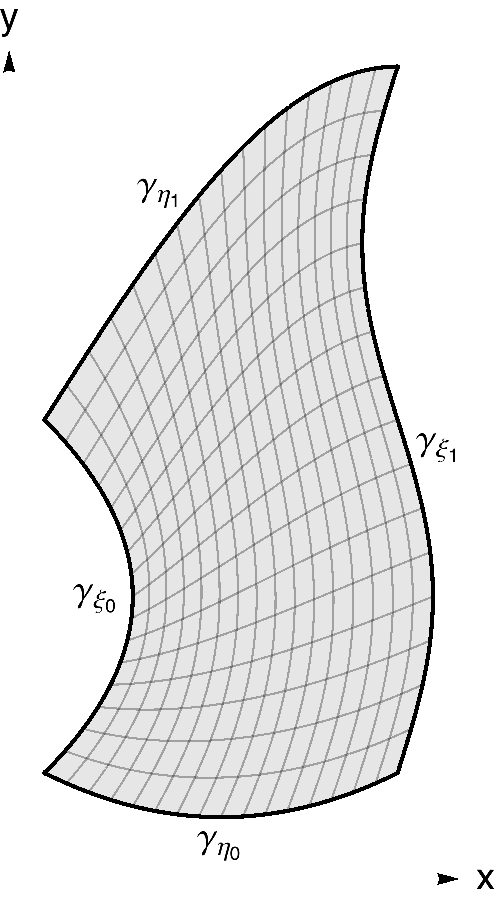
\includegraphics[width=.35\textwidth]{fig/testfig1.pdf}
\hspace{1cm}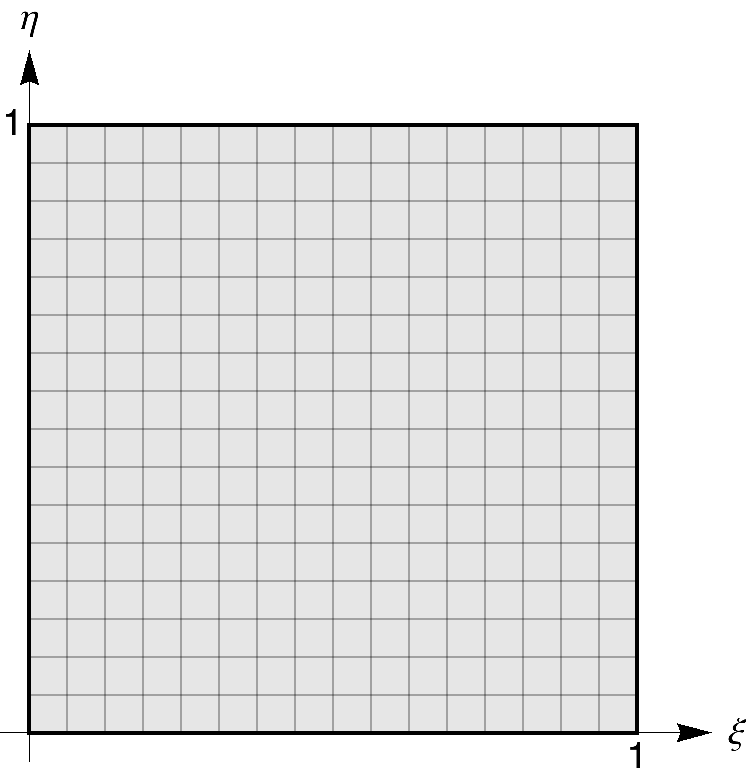
\includegraphics[width=.45\textwidth]{fig/testfig2.pdf}}
\caption{Figure Captions.}
\label{fig:label}
\end{figure}

\end{section}



%=== Appendix ============================================
\appendix

\dsp

\chapter{Appendix Title }{\label{appendix:a}}
\begin{section}{Section Title}

Appendicitis

\end{section}
\end{mainmatter}

%----- Bibliography ----------------
\ssp
\bibliographystyle{JHEP3}
\bibliography{thesis}

\end{document}
